\documentclass[12pt]{article}
\usepackage[utf8]{inputenc}
\usepackage[T5]{fontenc}
\usepackage{graphicx,a4wide,framed,amssymb}
\usepackage{tikz}
\usetikzlibrary{decorations,decorations.pathmorphing,shadows}

\newcommand{\source}[1]{\begin{flushright}\emph{[#1]}\end{flushright}}

\newcommand{\MakeScribeTop}[1]{
\noindent
\begin{framed}
\noindent
 Algorithmique Avancée 2018
 \hfill
 École Centrale-Supélec
 \\[1em]
 \centerline{ \Large
#1
 }
 \\[1em]
\centerline{  \it Christoph Dürr, Nguyễn Kim Thắng}
\end{framed}
}



\begin{document}
    \MakeScribeTop{PC4 : Flots et coupes 1}

\section{Couplage bi-parti de cardinalité maximum}

Vous êtes le père/la mère d'une très grande famille et vous voulez faire des cadeaux à vos enfants, qui sont au nombre de $n$.  Vous disposez de $m$ cadeaux.  Vous savez que certains cadeau ne conviennent pas à certains enfants. Concrètement vous disposez d'un graphe biparti $G(U,V,E)$ avec $|U|=n$, $|V|=m$, et $(u,v)\in E$ si le cadeau $v$ convient à l'enfant $u$.  Vous voulez trouvez un plus grand \emph{couplage} dans ce graphe, ce qui est défini par le plus grand ensemble $M\subseteq E$ tel que chaque sommet du graphe fasse parti d'au plus une arête de $M$. 


\begin{figure}[h]
	\centerline{
\includegraphics[width=2cm]{couplage.pdf}}
\end{figure}


Réduisez ce problème vers un problème de flot maximum.


\section{Élimination dans le baseball}


On est au milieu d'une compétition de baseball.
Je ne connais pas grand chose sur ce jeux, sauf que~:
\begin{itemize}
	\item Les matchs sont programmés en avance.
	\item Lors d'un match exactement une des deux équipes gagne.
	\item À la fin du tournoi chaque équipe a gagné un certain nombre de matchs. Ceux pour lesquelles ce nombre n'est pas maximum sont éliminées.
\end{itemize}

Dans l'exemple ci-dessous, Montréal sera éliminé, car même si elle gagne chacun des 3 matchs restants, elle n'arriverait qu'à atteindre 80 matchs gagnés, et Atlanta a déjà gagné plus que cela. Philly pourrait arriver à un score de 83, mais si Atlanta  perd tous ses matchs d'autres en gagneront, et finalement dépasseront Philly.

\begin{figure}[h]
	\centerline{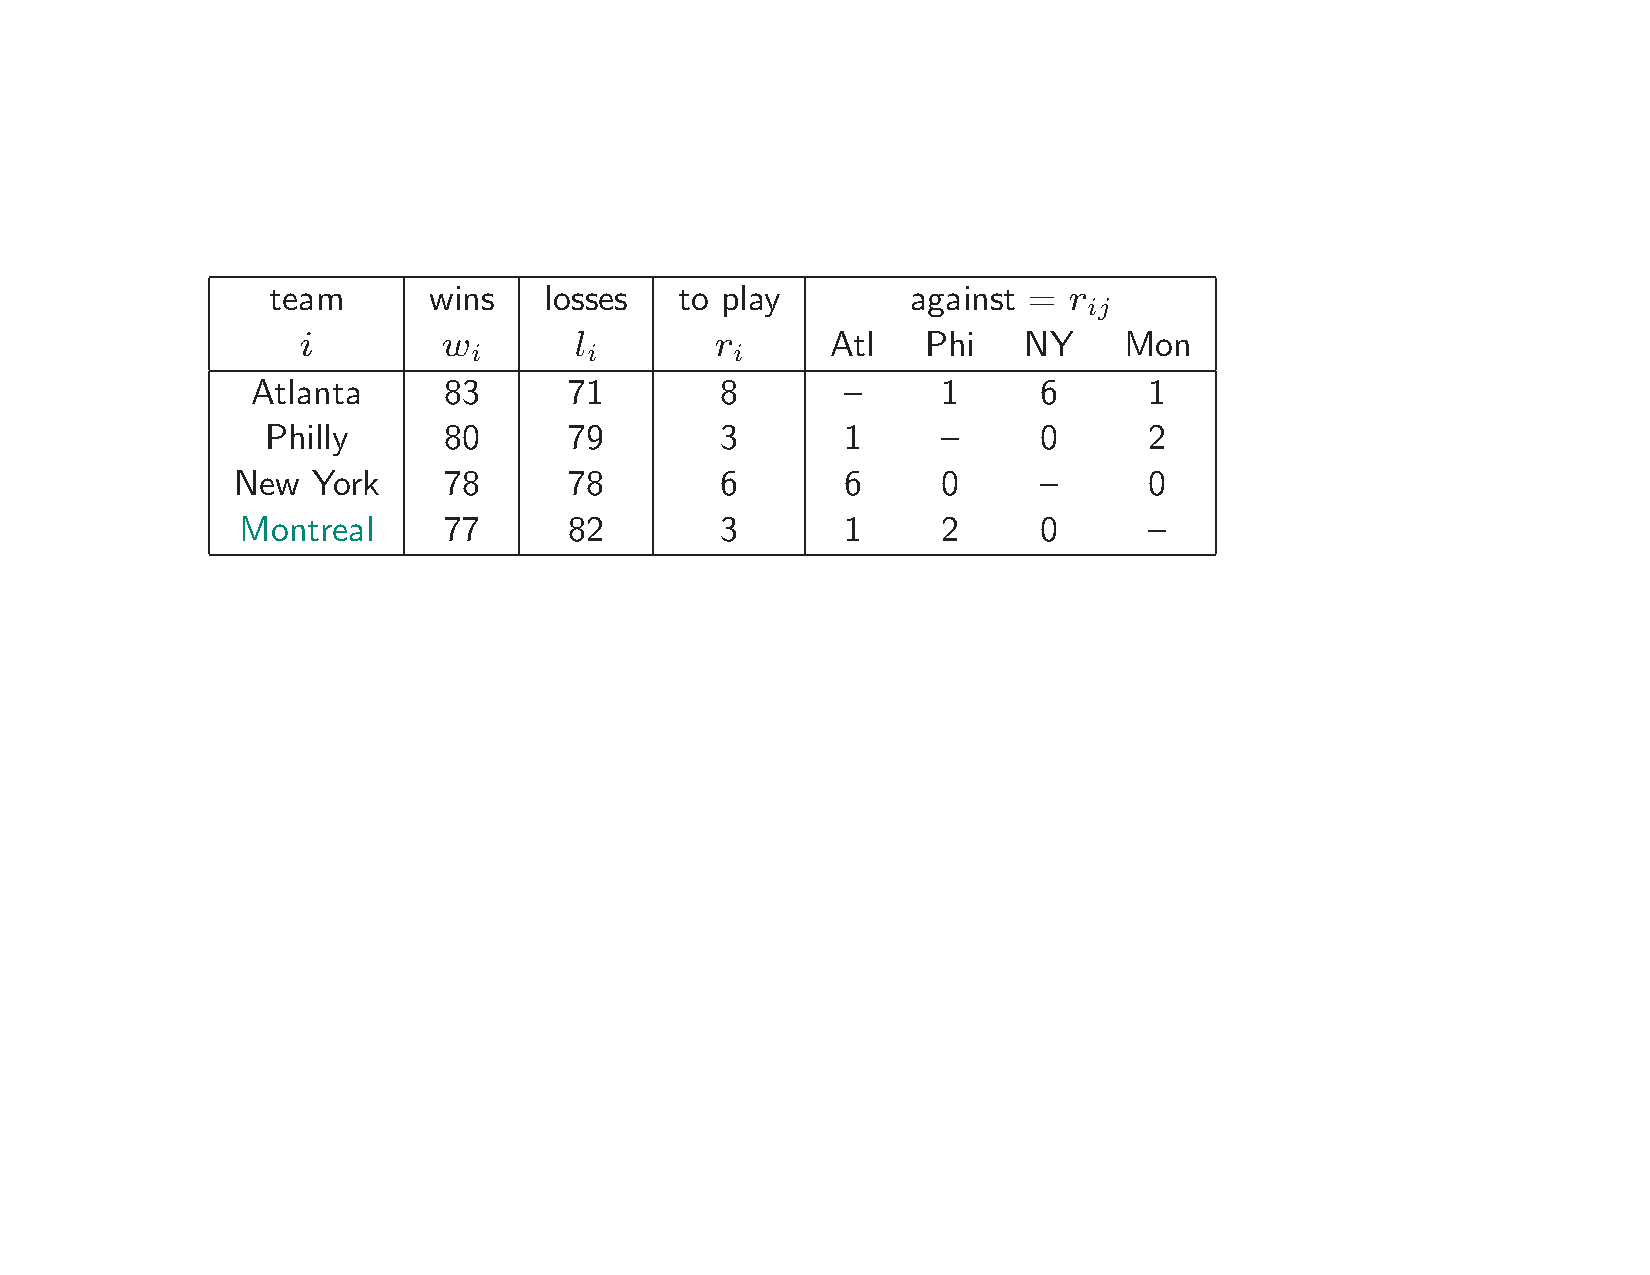
\includegraphics[width=12cm]{baseball.pdf}}
\end{figure}

Alors étant donnée $n$ équipes, le nombre $w_i$ de matchs déjà gagnés pour chaque équipe $i$, et la liste des matchs $(i,j)$ encore à jouer on cherche à déterminer si une équipe particulière $k$ a encore une chance de gagner.  Trouvez une réduction de ce problème à un problème de flot maximum. Indice: le graphe que vous allez construire ressemblera à celui de l'exercice précédent, mais avec d'autres capacités.

\section{Entrepreneur cupide}

Vous êtes un entrepreneur cupide, qui a reçu la commande de construire un bâtiment.  Ce travail se décompose en $n$ tâches, numérotés de $1$ à $n$. Ces tâches sont reliées par un ordre de précédence $\prec$, où $i\prec j$ dit que $j$ ne peut être effectuée seulement une fois $i$ est terminée.  Vous serez payé au fur et à mesure pour chaque tâche accomplie.  La tâche $i$ vous rapporte $w_i$ Euros, mais représente pour vous un coût de $p_i$ Euros. Vous n'avez pas du tout l'intention d'effectuer toutes les tâches, seulement un ensemble $S\subseteq \{1,\ldots, n\}$ avec la propriété que si $i\prec j$ et $j\in S$ alors $i\in S$ également.  On dit que l'ensemble est \emph{initial} pour l'ordre $\prec$.  Votre but est de trouver un ensemble initial $S$ qui maximise le ratio $(\sum_{i\in S} w_i )/ (\sum_{i\in S} p_i )$.

Trouvez une réduction de ce problème à un problème de flot maximum.  Indice: cherchez s'il existe une solution de ratio au moins $R$. Après vous pourriez faire une recherche dichotomique sur $R$.

\source{https://www.cs.princeton.edu/\~{}wayne/papers/baseball\_talk.pdf}
\end{document}